%!TEX root = main.tex
\setcounter{chapter}{2}
\setcounter{section}{4}
\setcounter{theorem}{0}
\setcounter{equation}{0}

\lectureheader{161}{Calculus I}{Limit practice}{\textit{Thomas' Calculus} 2.2 -- 2.4}

\begin{example}
Evaluate the limits or explain why they do not exist.
\begin{enumerate}
\item $\DS\lim_{x\to 1}\frac{|x-1|}{x-1}$
\vfill
\item $\DS\lim_{t\to 6}8(t-5)(t-7)$
\vfill
\item $\DS\lim_{y\to -3}(5-y)^{4/3}$
\vfill
\item $\DS\lim_{x\to 2}\frac{2x+5}{11-x^3}$
\vfill
\end{enumerate}
\end{example}

\newpage


\begin{example}
Evaluate the limits or explain why they do not exist.
\begin{enumerate}
\item $\DS\lim_{x\to -6}\frac{x+6}{x^2+4x-12}$
\vfill
\item $\DS\lim_{x\to 9}\frac{\sqrt x - 3}{x-9}$
\vfill
\item $\DS\lim_{x\to 0}\frac{\frac{1}{x-1}+\frac{1}{x+1}}{x}$
\vfill
\end{enumerate}
\end{example}

\newpage

\begin{example}
Evaluate the limits or explain why they do not exist.
\begin{enumerate}
\item $\DS\lim_{x\to 0}\cos(1/x)$
\vfill
\item $\DS\lim_{x\to 0}\sqrt x\sin(1/x)$
\vfill
\end{enumerate}
\end{example}

\newpage

\begin{example}
Evaluate the limits or explain why they do not exist.
\begin{enumerate}
\item $\DS\lim_{\theta\to 0}\frac{\tan\theta}{\theta^2\cot 3\theta}$
\vfill
\item $\DS\lim_{x\to 0}\frac{x+x\cos x}{\sin x\cos x}$
\vfill
\item $\DS\lim_{t\to 0}\frac{\sin(1-\cos t)}{1-\cos t}$
\vfill
\end{enumerate}
\end{example}

\newpage


\begin{example}
Your firm has been asked to supply the resistors for a circuit in which voltage $V$ will be 120 volts and current $I$ is to be 5 amps with a maximum deviation of $\epsilon=0.01$ amp.  
Compute the required resistance $R_0$ and maximum tolerance $\delta$ allowed. 
What if the circuit could only tolerate an $\epsilon=0.001$ amp deviation in the current?
Hint: Ohm's law states that $V=IR$.
\begin{flushright}
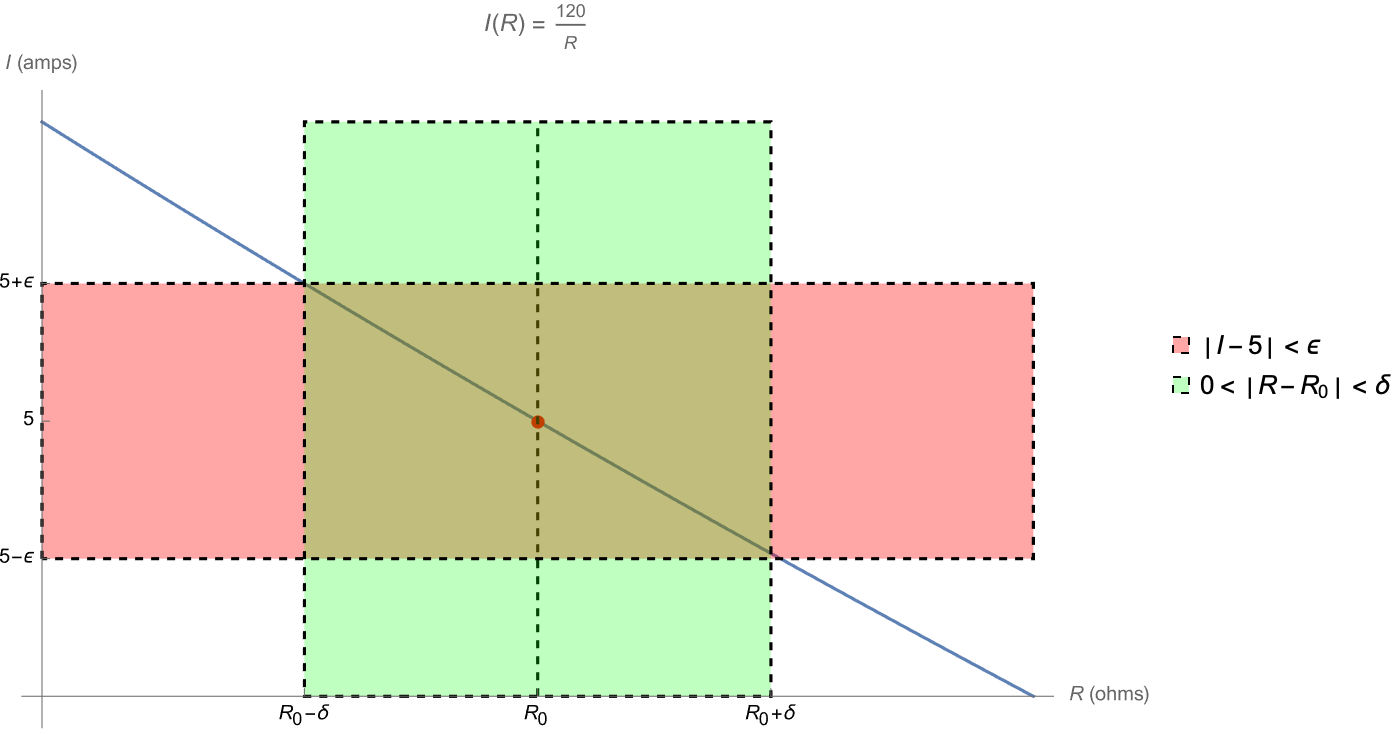
\includegraphics[width=3in]{img/tol_reg}
\end{flushright}
\end{example}

